\documentclass[border=10pt]{standalone}
\usepackage{tikz}
\usetikzlibrary{shapes.geometric, arrows.meta, positioning, calc, fit, backgrounds, shadows.blur, decorations.pathreplacing}
\usepackage[T1]{fontenc}
\usepackage{helvet}
\renewcommand{\familydefault}{\sfdefault}

\definecolor{morphorange}{HTML}{FF6B2B}
\definecolor{morphdark}{HTML}{0D0D1A}
\definecolor{morphgray}{HTML}{1A1A2E}
\definecolor{morphblue}{HTML}{4A90D9}
\definecolor{morphpurple}{HTML}{8B5CF6}
\definecolor{morphgreen}{HTML}{10B981}
\definecolor{morphaccent}{HTML}{F59E0B}
\definecolor{morphred}{HTML}{EF4444}
\definecolor{textwhite}{HTML}{F0F0F0}
\definecolor{textgray}{HTML}{9CA3AF}
\definecolor{cardbg}{HTML}{16162A}

\begin{document}
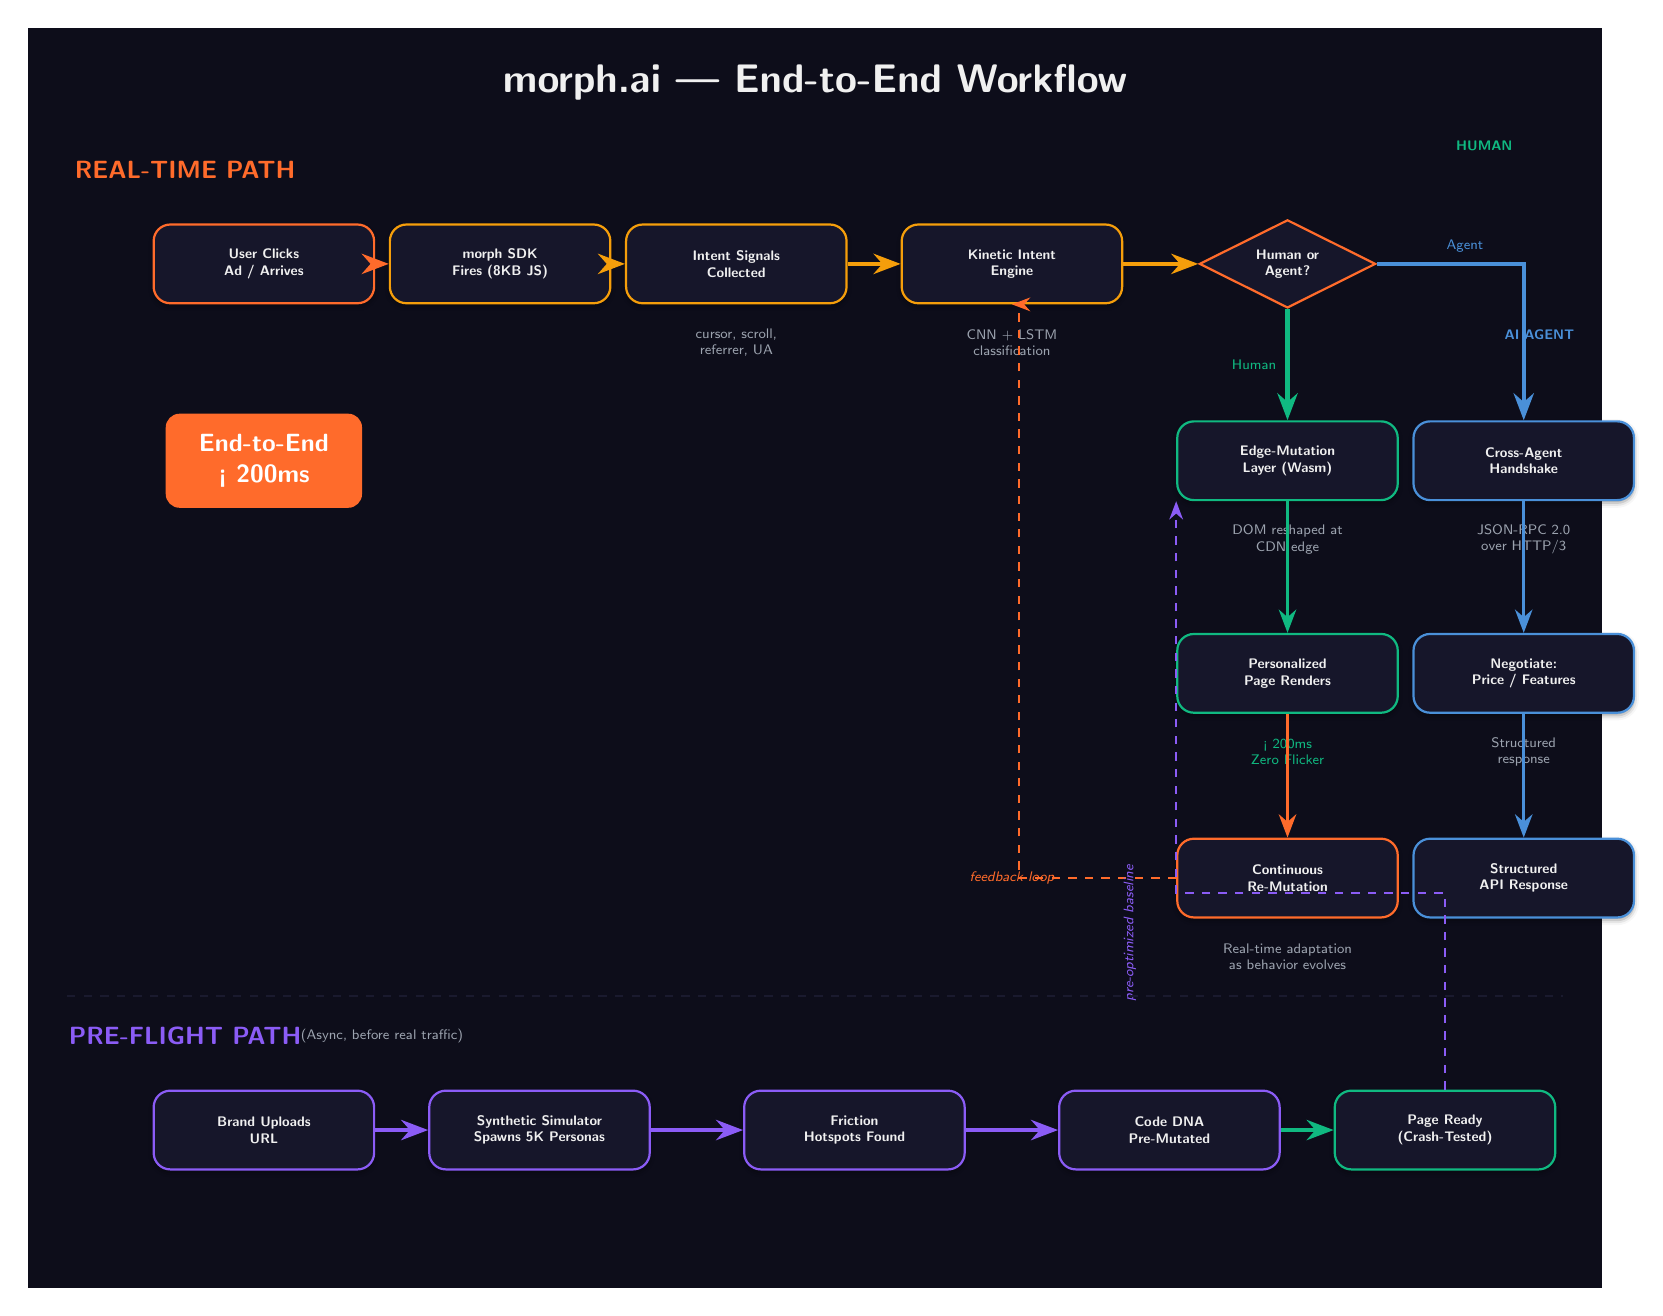
\begin{tikzpicture}[
    every node/.style={font=\sffamily},
    >=Stealth,
    process/.style={draw=#1, fill=cardbg, rounded corners=6pt, minimum width=2.8cm, minimum height=1cm,
                    text=textwhite, font=\sffamily\tiny\bfseries, line width=0.8pt, align=center,
                    blur shadow={shadow blur steps=3, shadow xshift=0pt, shadow yshift=-1pt}},
    decision/.style={draw=#1, fill=cardbg, diamond, aspect=2, minimum width=2cm, minimum height=1cm,
                     text=textwhite, font=\sffamily\tiny\bfseries, line width=0.8pt, align=center},
    label/.style={text=#1, font=\sffamily\tiny, align=center},
]

% Background
\fill[morphdark] (-10,-11) rectangle (10,5);

% Title
\node[text=textwhite, font=\sffamily\bfseries\Large] at (0,4.3) {morph.ai — End-to-End Workflow};

% =============================================
% TOP ROW: REAL-TIME PATH (Human + Agent)
% =============================================
\node[text=morphorange, font=\sffamily\bfseries\small] at (-8, 3.2) {REAL-TIME PATH};

% Step 1: User Clicks Ad
\node[process=morphorange] (click) at (-7, 2) {User Clicks\\Ad / Arrives};

% Step 2: SDK Fires
\node[process=morphaccent] (sdk) at (-4, 2) {morph SDK\\Fires (8KB JS)};

% Step 3: Signal Collection
\node[process=morphaccent] (signals) at (-1, 2) {Intent Signals\\Collected};
\node[label=textgray] at (-1, 1.0) {cursor, scroll,\\referrer, UA};

% Step 4: Classification
\node[process=morphaccent] (classify) at (2.5, 2) {Kinetic Intent\\Engine};
\node[label=textgray] at (2.5, 1.0) {CNN + LSTM\\classification};

% Step 5: Decision Diamond
\node[decision=morphorange] (decide) at (6, 2) {Human or\\Agent?};

% === HUMAN PATH (upper) ===
\node[text=morphgreen, font=\sffamily\bfseries\tiny] at (8.5, 3.5) {HUMAN};

\node[process=morphgreen] (edgemut) at (6, -0.5) {Edge-Mutation\\Layer (Wasm)};
\node[label=textgray] at (6, -1.5) {DOM reshaped at\\CDN edge};

\node[process=morphgreen] (render) at (6, -3.2) {Personalized\\Page Renders};
\node[label=morphgreen] at (6, -4.2) {< 200ms\\Zero Flicker};

\node[process=morphorange] (adapt) at (6, -5.8) {Continuous\\Re-Mutation};
\node[label=textgray] at (6, -6.8) {Real-time adaptation\\as behavior evolves};

% === AGENT PATH (right) ===
\node[text=morphblue, font=\sffamily\bfseries\tiny] at (9.2, 1.1) {AI AGENT};

\node[process=morphblue] (handshake) at (9, -0.5) {Cross-Agent\\Handshake};
\node[label=textgray] at (9, -1.5) {JSON-RPC 2.0\\over HTTP/3};

\node[process=morphblue] (negotiate) at (9, -3.2) {Negotiate:\\Price / Features};
\node[label=textgray] at (9, -4.2) {Structured\\response};

\node[process=morphblue] (agentresp) at (9, -5.8) {Structured\\API Response};

% === ARROWS: Real-Time Path ===
\draw[->, morphorange, line width=1.5pt] (click) -- (sdk);
\draw[->, morphaccent, line width=1.5pt] (sdk) -- (signals);
\draw[->, morphaccent, line width=1.5pt] (signals) -- (classify);
\draw[->, morphaccent, line width=1.5pt] (classify) -- (decide);

% Decision branches
\draw[->, morphgreen, line width=1.5pt] (decide.south) -- node[left, label=morphgreen] {Human} (edgemut.north);
\draw[->, morphblue, line width=1.5pt] (decide.east) -| node[above, label=morphblue, pos=0.3] {Agent} (handshake.north);

% Human path flow
\draw[->, morphgreen, line width=1.2pt] (edgemut) -- (render);
\draw[->, morphorange, line width=1.2pt] (render) -- (adapt);

% Feedback loop
\draw[->, morphorange, line width=0.8pt, dashed] (adapt.west) -- ++(-2,0) |- (classify.south);
\node[text=morphorange, font=\sffamily\tiny\itshape] at (2.5, -5.8) {feedback loop};

% Agent path flow
\draw[->, morphblue, line width=1.2pt] (handshake) -- (negotiate);
\draw[->, morphblue, line width=1.2pt] (negotiate) -- (agentresp);

% =============================================
% BOTTOM: PRE-FLIGHT PATH (Async)
% =============================================
\node[text=morphpurple, font=\sffamily\bfseries\small] at (-8, -7.8) {PRE-FLIGHT PATH};
\node[text=textgray, font=\sffamily\tiny] at (-5.5, -7.8) {(Async, before real traffic)};

\node[process=morphpurple] (upload) at (-7, -9) {Brand Uploads\\URL};

\node[process=morphpurple] (spawn) at (-3.5, -9) {Synthetic Simulator\\Spawns 5K Personas};

\node[process=morphpurple] (friction) at (0.5, -9) {Friction\\Hotspots Found};

\node[process=morphpurple] (premut) at (4.5, -9) {Code DNA\\Pre-Mutated};

\node[process=morphgreen] (ready) at (8, -9) {Page Ready\\(Crash-Tested)};

% Pre-flight arrows
\draw[->, morphpurple, line width=1.5pt] (upload) -- (spawn);
\draw[->, morphpurple, line width=1.5pt] (spawn) -- (friction);
\draw[->, morphpurple, line width=1.5pt] (friction) -- (premut);
\draw[->, morphgreen, line width=1.5pt] (premut) -- (ready);

% Connect pre-flight to real-time
\draw[->, morphpurple, line width=0.8pt, dashed] (ready.north) -- ++(0,2.5) -| (edgemut.south west);
\node[text=morphpurple, font=\sffamily\tiny\itshape, rotate=90] at (4.0, -6.5) {pre-optimized baseline};

% === Separator line ===
\draw[morphgray, line width=0.5pt, dashed] (-9.5, -7.3) -- (9.5, -7.3);

% === Latency callout ===
\node[fill=morphorange, rounded corners=5pt, text=white, font=\sffamily\bfseries\small, inner sep=6pt] 
      at (-7, -0.5) {\begin{tabular}{c}End-to-End\\< 200ms\end{tabular}};

\end{tikzpicture}
\end{document}
